%----------------------------------------------------------------------------------------
%	PACKAGES AND THEMES
%----------------------------------------------------------------------------------------

\documentclass{beamer}
\mode<presentation> {
	\usetheme{Warsaw}
	\setbeamercolor{page_num_color}{fg=white,bg=blue}

	\defbeamertemplate*{footline}{shadow theme}{%
		\leavevmode%
		\hbox{\begin{beamercolorbox}[wd=.5\paperwidth,ht=2.5ex,dp=1.125ex,leftskip=.3cm plus1fil,rightskip=.3cm]{author in head/foot}%
		    \usebeamerfont{author in head/foot}\hfill\insertshortauthor
		\end{beamercolorbox}%
		\begin{beamercolorbox}[wd=.4\paperwidth,ht=2.5ex,dp=1.125ex,leftskip=.3cm,rightskip=.3cm plus1fil]{title in head/foot}%
		    \usebeamerfont{title in head/foot}\insertshorttitle\hfill%
		\end{beamercolorbox}%
		\begin{beamercolorbox}[wd=.1\paperwidth,ht=2.5ex,dp=1.125ex,leftskip=.3cm,rightskip=.3cm plus1fil]{author in head/foot}%
		\hfill\insertframenumber\,/\,\inserttotalframenumber
		\end{beamercolorbox}}%
		\vskip0pt%
	}
}

\usepackage{mathrsfs}
\usepackage{amsmath}
\usepackage{amssymb}
\usepackage{graphicx} % Allows including images
\usepackage{booktabs} % Allows the use of \toprule, \midrule and \bottomrule in tables
\usepackage[english]{babel}
\usepackage{graphicx}
\usepackage{listings, lstautogobble}
\usepackage{color}
\usepackage{caption}
\usepackage{verbatim}


%----------------------------------------------------------------------------------------
%	LSTSETTING
%----------------------------------------------------------------------------------------
\lstset{language=C,
    keywordstyle=\color{blue}, 
    morekeywords={then},
    numberstyle=\footnotesize,
    basicstyle=\ttfamily\footnotesize,
    numbers=left,
    stepnumber=1,
    frame=single,
    breaklines=true,
    tabsize=4,
    escapeinside={(*}{*)},
    autogobble=true
}

%----------------------------------------------------------------------------------------
%   TITLE PAGE 
%----------------------------------------------------------------------------------------

\title[Toward Resource-Efficient Cloud Systems]
{Toward Resource-Efficient Cloud Systems: Avoiding Over-Provisioning in Demand-Prediction Based Resource Provisioning} % The short title appears at the bottom of every slide, the full title is only on the title page
\author[Liuhua Chen, Haiying Shen]
{   Liuhua Chen \\
	{\it ECE, Clemson University} \\
	Haiying Shen \\
	{\it CS, University of Virginia}
} % Your name
\institute[] % Your institution as it will appear on the bottom of every slide, may be shorthand to save space
{
	2016 IEEE International Conference on Big Data \\ % Your institution for the title page
 	\bigskip Presenter: Yi-Ning Chang
}
\date{October 19, 2017} % Date, can be changed to a custom date


\begin{document}

%----------------------------------------------------------------------------------------
%	TITLE PAGE SETTING
%----------------------------------------------------------------------------------------
\begin{frame}[noframenumbering]
    \titlepage % Print the title page as the first slide
\end{frame}

\AtBeginSection[]
  {
  	 \setbeamertemplate{footline}{} 
     \begin{frame}<beamer>[noframenumbering]
     \tableofcontents[currentsection, hideallsubsections]
     \end{frame}
     \setbeamertemplate{footline}{%
		\leavevmode%
		\hbox{\begin{beamercolorbox}[wd=.5\paperwidth,ht=2.5ex,dp=1.125ex,leftskip=.3cm plus1fil,rightskip=.3cm]{author in head/foot}%
		    \usebeamerfont{author in head/foot}\hfill\insertshortauthor
		\end{beamercolorbox}%
		\begin{beamercolorbox}[wd=.4\paperwidth,ht=2.5ex,dp=1.125ex,leftskip=.3cm,rightskip=.3cm plus1fil]{title in head/foot}%
		    \usebeamerfont{title in head/foot}\insertshorttitle\hfill%
		\end{beamercolorbox}%
		\begin{beamercolorbox}[wd=.1\paperwidth,ht=2.5ex,dp=1.125ex,leftskip=.3cm,rightskip=.3cm plus1fil]{author in head/foot}%
		\hfill\insertframenumber\,/\,\inserttotalframenumber
		\end{beamercolorbox}}%
		\vskip0pt%
	}
  }


%------------------------------------------------
% Outline
%------------------------------------------------
\begin{frame}
\frametitle{Outline} % Table of contents slide, comment this block out to remove it
\tableofcontents[hideallsubsections] % Throughout your presentation, if you choose to use \section{} and \subsection{} commands, these will automatically be printed on this slide as an overview of your presentation
\end{frame}


%------------------------------------------------
% Introduction
%------------------------------------------------
\section{Introduction}

% Introduction
\subsection{Introduction}
    \begin{frame}
    \frametitle{Introduction}
		\begin{itemize}
		\item In cloud systems, cloud providers abstract resources in physical machines into virtual machines and sell them to the tenants.
		\item To ensure resource provisioning for guaranteeing SLOs\footnotemark[1], clouds can use {\it demand-prediction based resource provisioning schemes}.
		\item Achieving the tradeoff between the penalties associated with {\it SLO violations} and {\it high resource utilization} requires an accurate demand prediction methodology.
		\end{itemize}
		\footnotetext[1]{SLO: Service Level Objectives}
    \end{frame}

% CloudScale
\subsection{Previous Work}
	\begin{frame}
	\frametitle{Previous Work - CloudScale}
		\begin{figure}[h!]
		\centering
		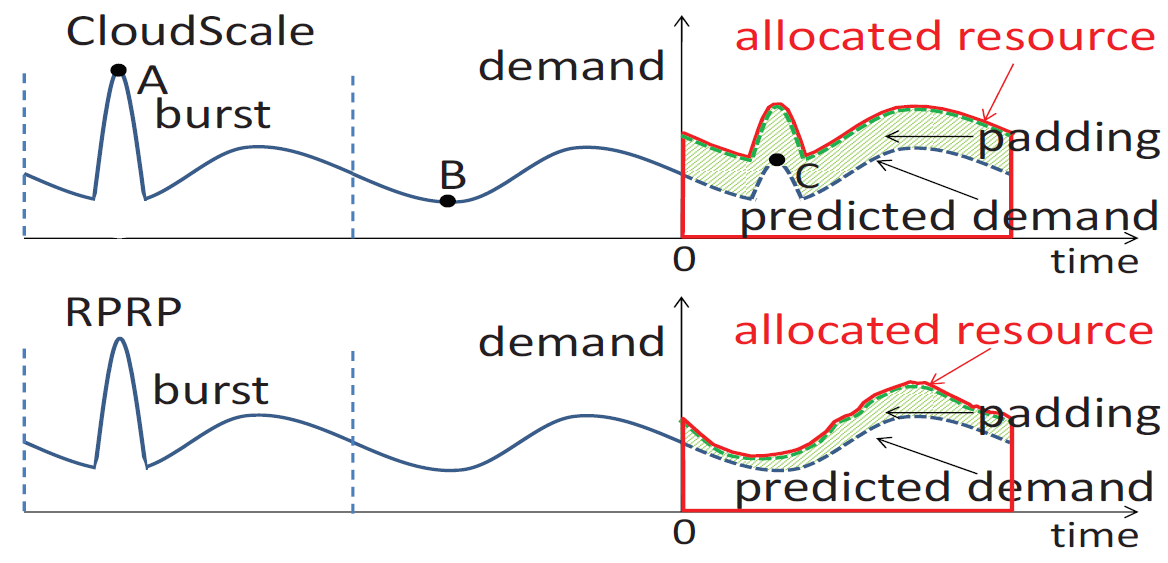
\includegraphics[width=0.6\textwidth]{./figure/intro.PNG}
		\end{figure}
		\begin{itemize}
		\item CloudScale predicts the demand at a time period based on a historical record.
		\item Padding: using the high-frequency spectrum or the average of the latest prediction error.
		\item Online Adaptive: to handle underestimation, raising the resource allocation by $\alpha>1$ until an error is corrected.
		\end{itemize}
	\end{frame}

% RPRP
\subsection{RPRP}
	\begin{frame}
	\frametitle{RPRP\footnotemark[1]}
		\begin{itemize}
		\item RPRP excludes bursts in demand prediction and specifically handles bursts to avoid resource over-provisioning.
		\item Algorithm
			\begin{itemize}
			\item {\it burst-exclusive prediction algorithm}
			\item {\it load-dependent padding algorithm}
			\item {\it responsive padding algorithm}
			\end{itemize}
		\item Algorithm 1 and 2 aim to exclude bursts, and algorithm 3 aims to handle bursts.
		\end{itemize}
		\footnotetext[1]{RPRP: Resource-efficient Predictive Resource Provisioning system}
	\end{frame}

%------------------------------------------------
% System Design
%------------------------------------------------
\section{System Design}

% Objective
\subsection{Objective}
	\begin{frame}
	\frametitle{Objective}
		\begin{itemize}
		\item Denote a VM's records:
			\begin{itemize}
			\item {\it workload demand}: $D=\{d_{t_{1}},...,d_{t_{i}},...,d_{t_{N}}\}$
			\item {\it allocated resource}: $A=\{a_{t_{1}},...,a_{t_{i}},...,a_{t_{N}}\}$
			\item {\it utilized resource}: $U=\{u_{t_{1}},...,u_{t_{i}},...,u_{t_{N}}\}$
			\item {\it resource capacity}: $C$
			\end{itemize}
		\item And from the historical records, we have:
			\begin{itemize}
			\item {\it predict demand}: $P=\{p_{t_{N+1}},p_{t_{N+2}},...,p_{t_{N+T}}\}$
			\item {\it allocated resource}: $A=\{a_{t_{N+1}},a_{t_{N+2}},...,a_{t_{N+T}}\}$
			\end{itemize}
		\item Goal: determine allocated resource $A$ such that
			\begin{itemize}
			\item $d_{t_{i}} \leq a_{t_{i}} \leq C$
			\item and meanwhile to minimize $a_{t_{i}}-d_{t_{i}}, \forall t_{i} > t_{N}$
			\end{itemize}
		\end{itemize}
	\end{frame}

% Algorithm
\subsection{Algorithm}

	% Burst-exclusive Prediction
	\begin{frame}
	\frametitle{Algo.1: Burst-exclusive Prediction}
		\begin{itemize}
		\item Trace analysis and CloudScale prediction $+$ padding.
		\end{itemize}
		\begin{figure}[h!]
		\centering
		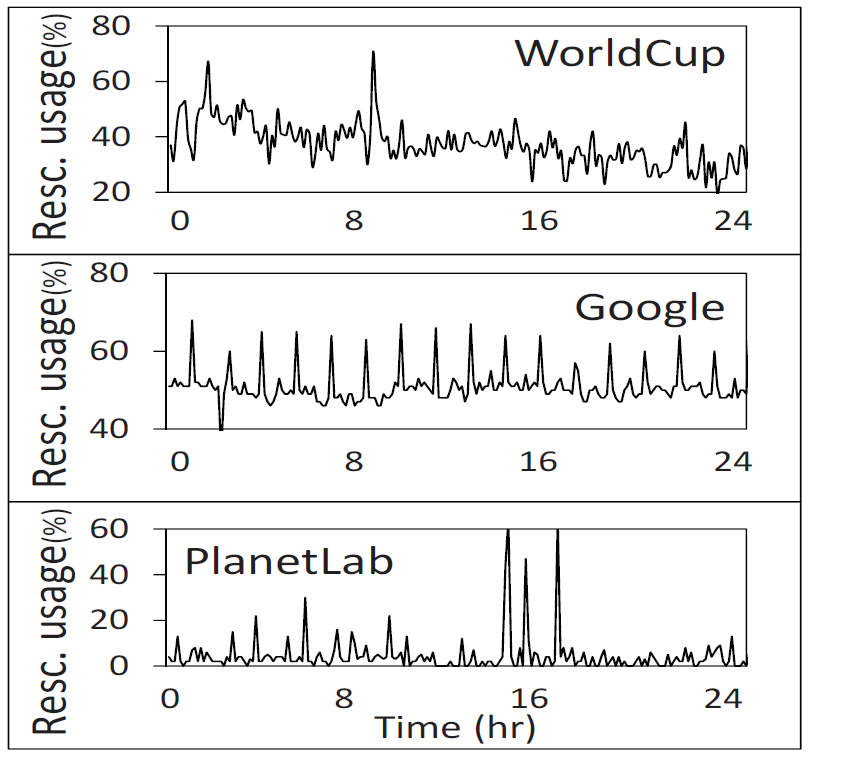
\includegraphics[width=0.4\textwidth]{./figure/alg1_1.PNG}
		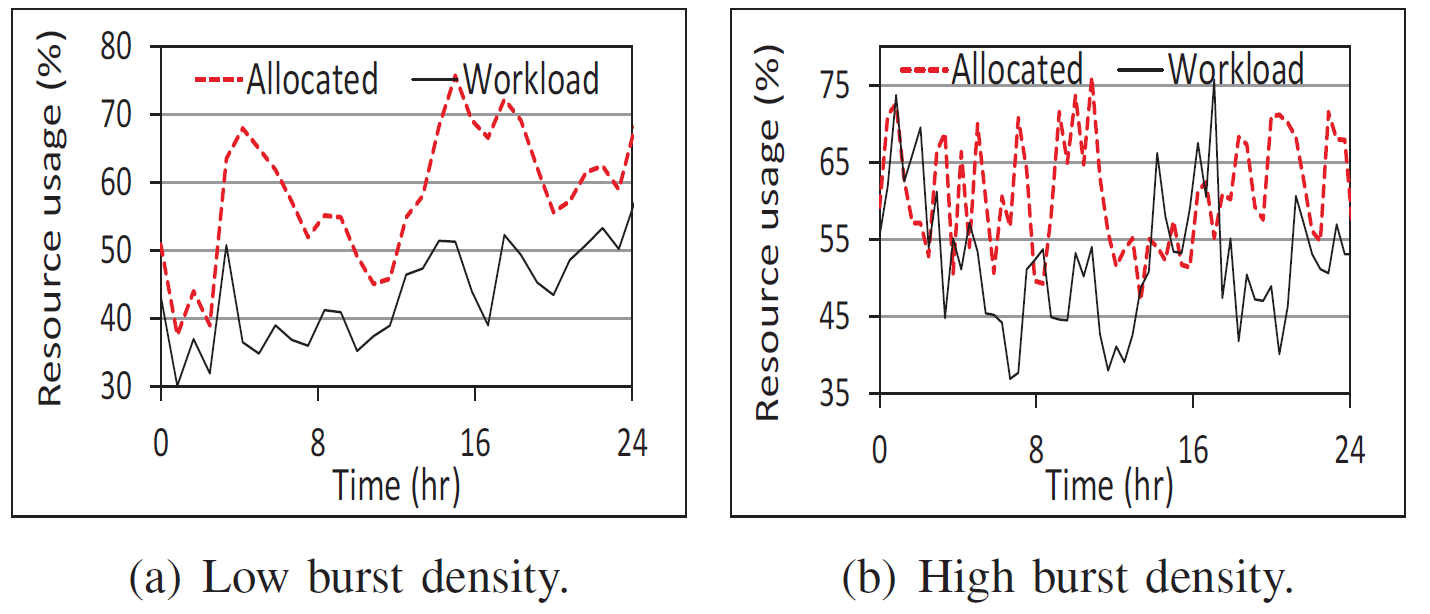
\includegraphics[width=0.6\textwidth]{./figure/alg1_2.PNG}
		\end{figure}
	\end{frame}

	\begin{frame}
	\frametitle{Algo.1: Burst-exclusive Prediction}
		\begin{itemize}
		\item RPRP relies on FFT to exclude the burst.
		\item FFT is applicable for predicting workload demand in repeated periodic patterns $P$ based on the historical utilization series $U$.
		\end{itemize}
		\begin{figure}[h!]
		\centering
		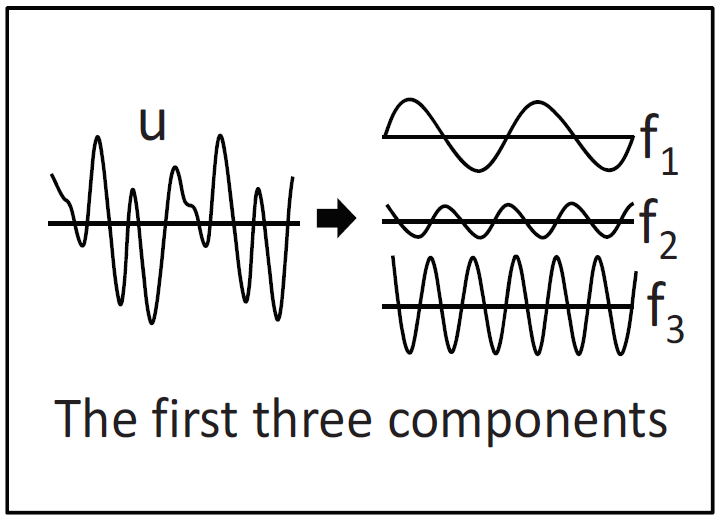
\includegraphics[width=0.4\textwidth]{./figure/alg1_3.PNG}
		\end{figure}
	\end{frame}

	% Load-dependent Padding
	\begin{frame}
	\frametitle{Algo.2: Load-dependent Padding}
		\begin{itemize}
		\item Formulate the problem of padding determination to achieve both {\it resource efficient} and {\it SLO guarantee}.
		\item The variation of prediction errors is dependent on load levels in cloud.
		\item Use $\mathscr{P}=\{\hat{p_{1}}, \hat{p_{2}}, ..., \hat{p_{M}}\}$ ($\hat{p_{1}} < \hat{p_{2}} < ... < \hat{p_{M}}$) to represent the M different predicted demand levels.
		\item Use $\mathscr{D}_{\hat{P_{i}}}=\{d_{1}, d_{2}, ..., d_{n_{\hat{p_{i}}}}\}$ ($d_{1} < d_{2} < ... < d_{n_{\hat{p_{i}}}},n_{\hat{p_{i}}}=\mid{\mathscr{D}_{\hat{p_{i}}}}\mid$) to indicate the demands that were predicted to be $\hat{p_{i}}$.
		\item And $N = \sum_{j=1}^{M} n_{\hat{p_{j}}}$ is the total number of workload demands in the demand series.
		\end{itemize}
	\end{frame}

	\begin{frame}
	\frametitle{Algo.2: Load-dependent Padding}
		\begin{itemize}
		\item The probability that the allocated resource ($a_{t_{i}}=\hat{p_{i}}+\delta(\hat{p_{i}})$) is sufficient to meet the demand is
		\end{itemize}
		\begin{equation} Pr(\hat{p_{i}})=\frac{\mid \{ d_{j}\leq\hat{p_{i}}+\delta(\hat{p_{i}}) \mid d_{j}\in \mathscr{D}_{\hat{p_{i}}} \} \mid}{n_{\hat{p_{i}}}} \end{equation}
		\begin{equation} \bar{Pr}=\sum^{M}_{i=1}Pr(\hat{p_{i}})\frac{n_{\hat{p_{i}}}}{N}=\sum^{M}_{i=1}\frac{\mid \{ d_{j}\leq\hat{p_{i}}+\delta(\hat{p_{i}}) \mid d_{j}\in \mathscr{D}_{\hat{p_{i}}} \} \mid}{n_{\hat{p_{i}}}} \frac{n_{\hat{p_{i}}}}{N} \geq 1-\epsilon \end{equation}
		\begin{itemize}
		\item The expected allocated resource amount can be calculated by
		\end{itemize}
		\begin{equation} \sum_{\hat{p_{i}}\in\mathscr{P}}[\hat{p_{i}}+\delta(\hat{p_{i}})]\frac{n_{\hat{p_{i}}}}{N} \end{equation}
	\end{frame}

	\begin{frame}
	\frametitle{Algo.2: Load-dependent Padding}
		\begin{figure}[h!]
		\centering
		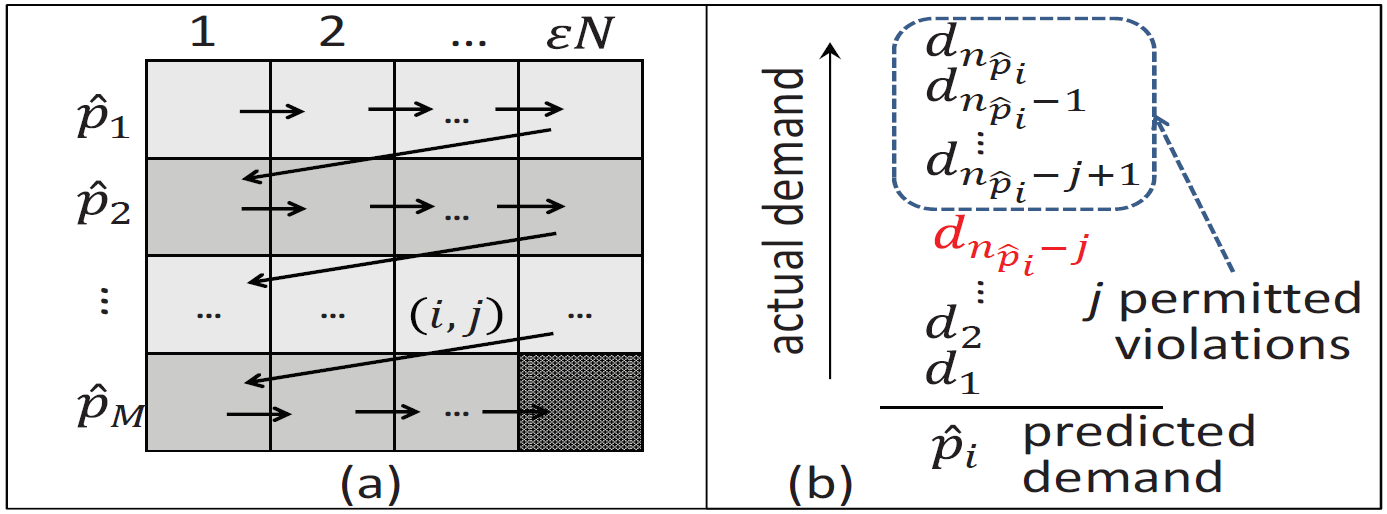
\includegraphics[width=0.7\textwidth]{./figure/alg2_1.PNG}
		\end{figure}
		\begin{itemize}
		\item Solved by an $M\times \epsilon N$ dynamics programming.
		\item In the matrix, $\mathbb{M}(i,j)$ represents the minimum total allocated resource when distributing $j$ violations to the first $i$ predicted demand levels.
		\item $\mathbb{M}(i,j)=min_{0<x<j}\{ \mathbb{M}(i-1,j-1)+d_{n_{\hat{p_{i}}}-x}\times n_{\hat{p_{i}}} \}$
		\end{itemize}
	\end{frame}

	% Responsive Padding
	\begin{frame}
	\frametitle{Algo.3: Responsive Padding}
		\begin{figure}[h!]
		\centering
		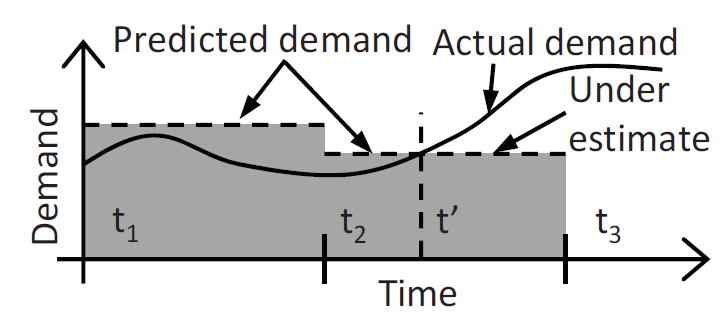
\includegraphics[width=0.4\textwidth]{./figure/alg3_1.PNG}
		\end{figure}
		\begin{itemize}
		\item If the resource utilization is upper than $T_{u}$ at time $t'$, then
		\begin{equation} a_{t'+\Delta}=a_{t'}+\frac{1}{2}(u_{max}-a_{t'}) \end{equation}
		\item If the resource utilization is lower than $T_{l}$ after raising, then
		\begin{equation} a_{t''+\Delta}=a_{t''}-\frac{1}{2}(a_{t''}-u_{t''}) \end{equation}
		\item $T_{l}$, $T_{u}$ are lower and upper bound threshold.
		\item $u_{max}$ is the maximum recorded utilization.
		\item $\Delta$ is a monitoring interval.
		\end{itemize}
	\end{frame}

%------------------------------------------------
% Evaluation
%------------------------------------------------
\section{Evaluation}

% Analytical Performance Evaluation
\subsection{Analytical Performance Evaluation}
	\begin{frame}
	\frametitle{Performance of Burst-exclusive Prediction}
		\begin{figure}[h!]
		\centering
		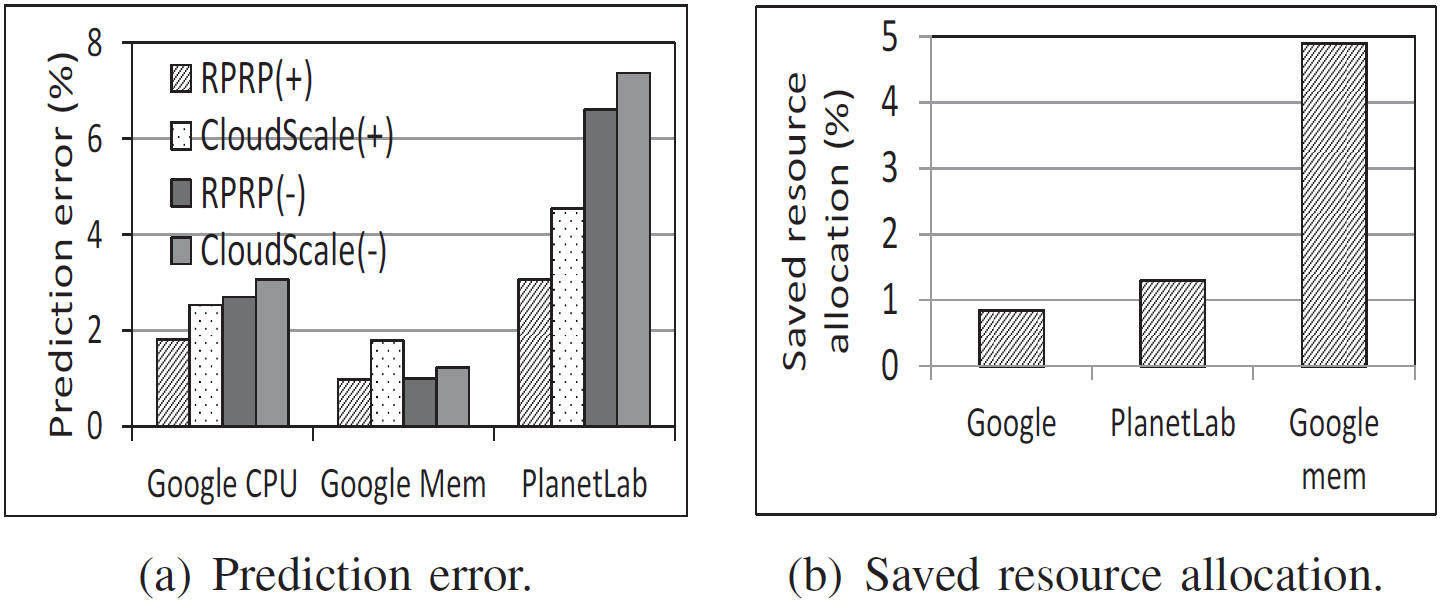
\includegraphics[width=0.7\textwidth]{./figure/eva1_1.PNG}
		\end{figure}
		\begin{itemize}
		\item Average prediction error is calculated by $\frac{1}{n}\sum_{i=1}^{n}\mid \hat{p_{i}}-d_{i} \mid$
		\item Saved resource allocation is calculated by $\frac{CloudScale-RPRP}{CloudScale}$
		\end{itemize}
	\end{frame}

	\begin{frame}
	\frametitle{Perfornmance of Load-dependent Padding}
		\begin{figure}[h!]
		\centering
		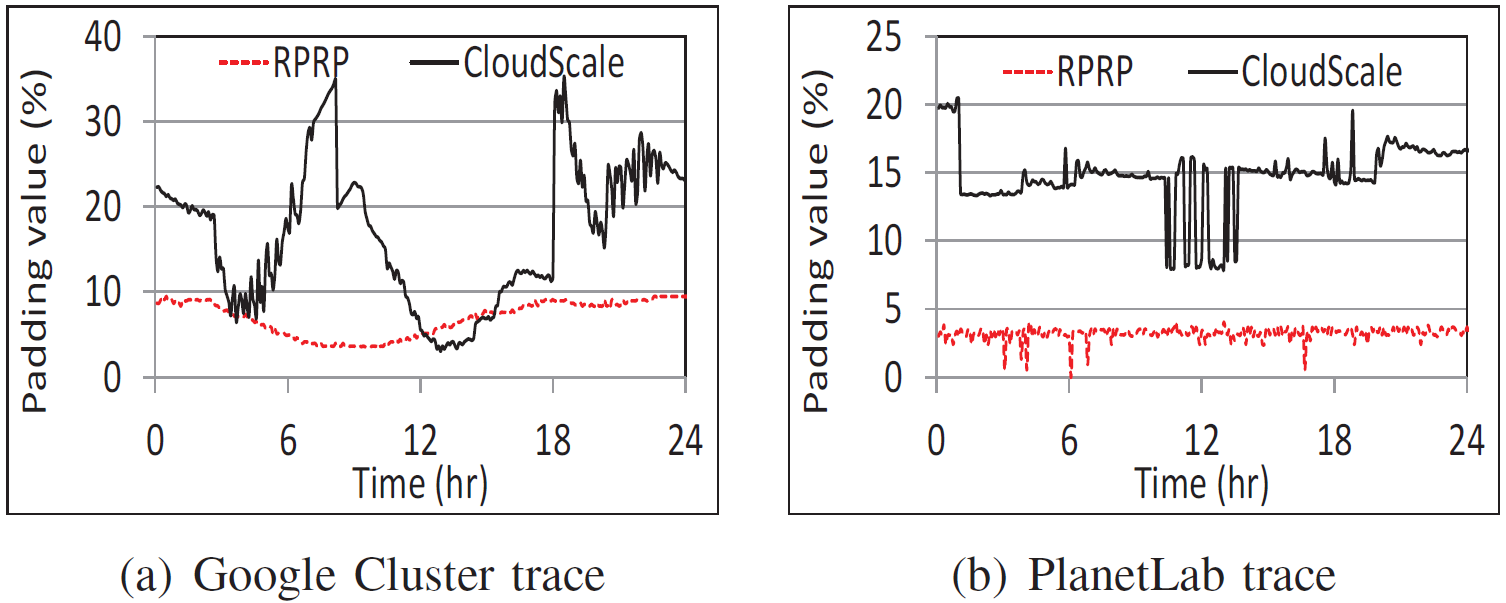
\includegraphics[width=0.7\textwidth]{./figure/eva1_2.PNG}
		\end{figure}
		\begin{figure}[h!]
		\centering
		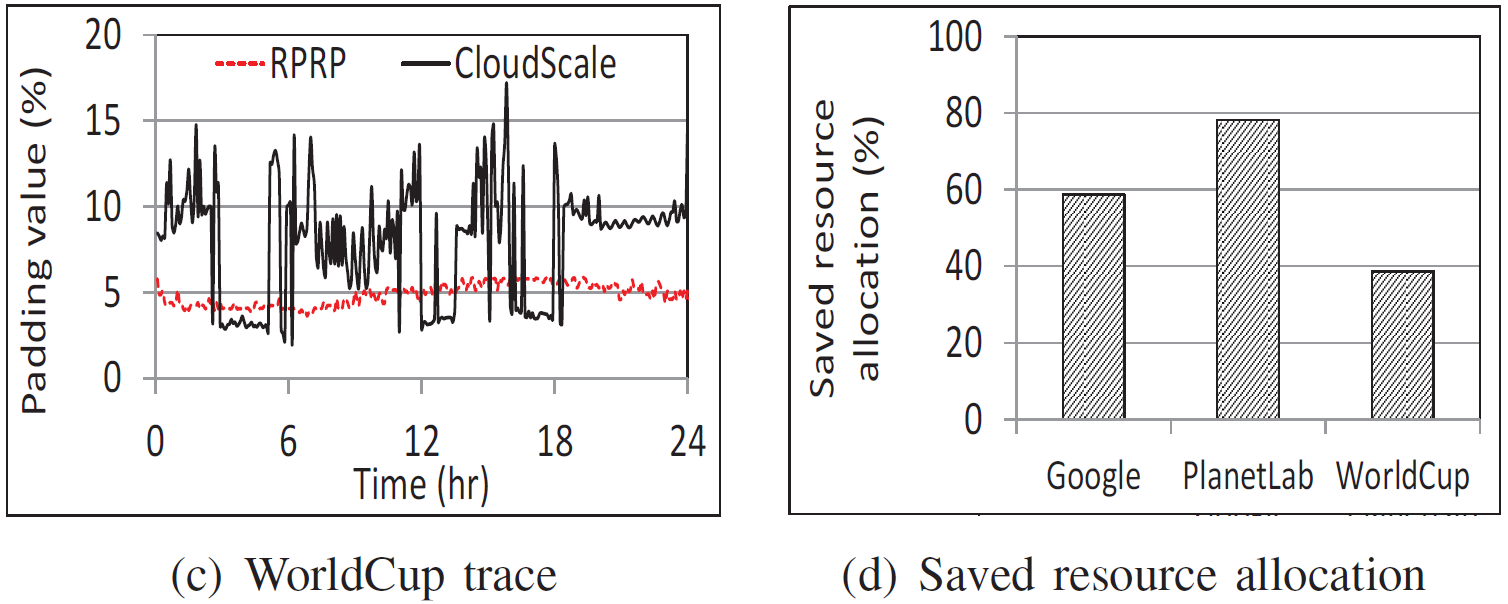
\includegraphics[width=0.7\textwidth]{./figure/eva1_3.PNG}
		\end{figure}
	\end{frame}

	\begin{frame}
	\frametitle{Perfornmance of Resource Provisioning}
		\begin{figure}[h!]
		\centering
		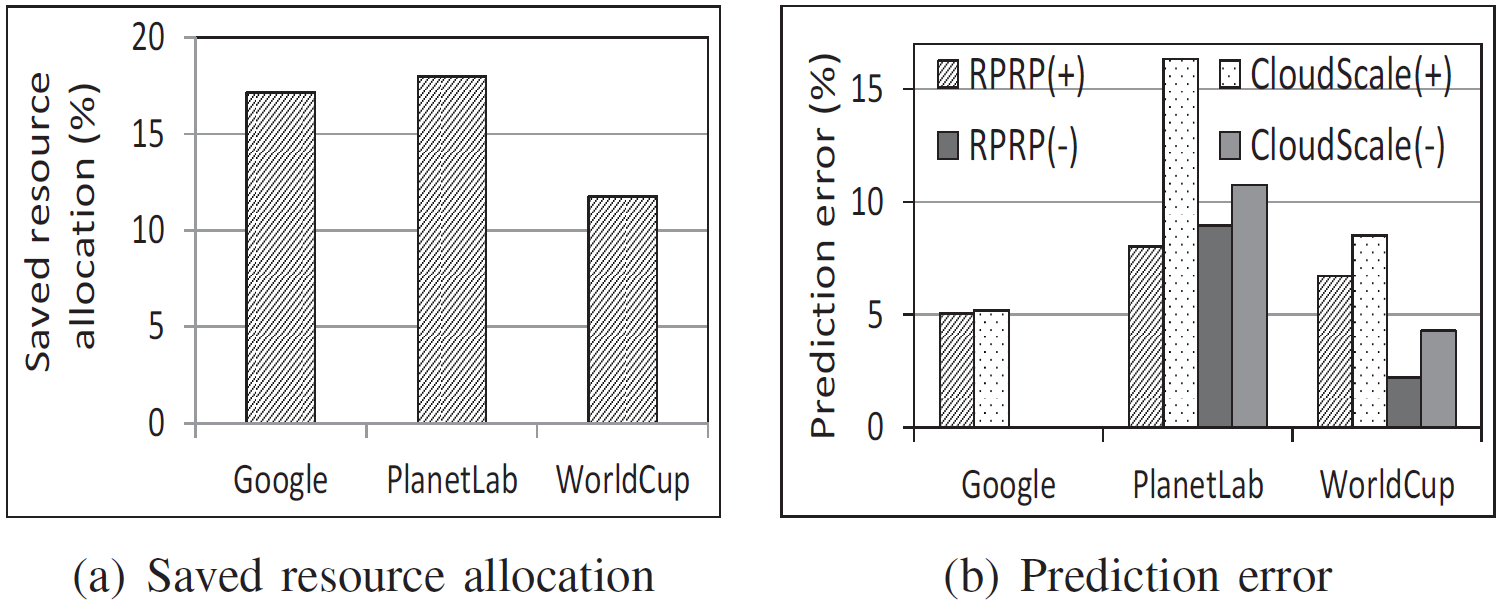
\includegraphics[width=0.7\textwidth]{./figure/eva1_4.PNG}
		\end{figure}
		\begin{figure}[h!]
		\centering
		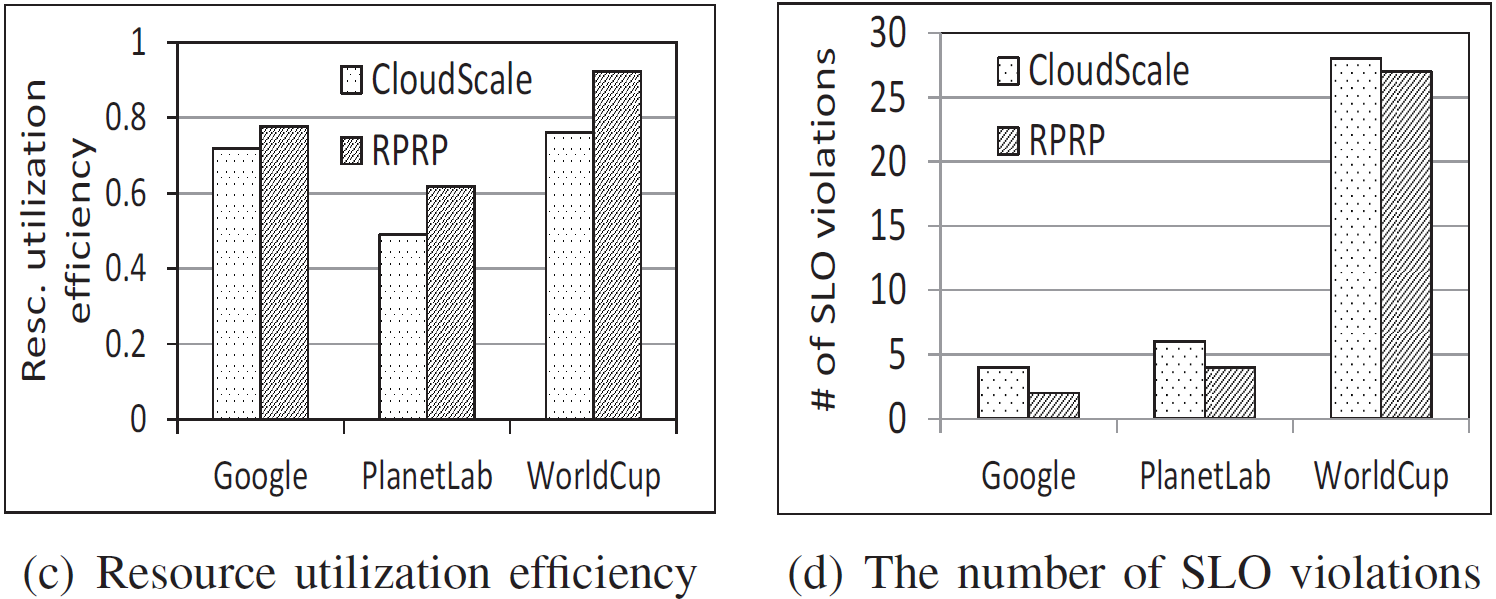
\includegraphics[width=0.7\textwidth]{./figure/eva1_5.PNG}
		\end{figure}
	\end{frame}

	\begin{frame}
	\frametitle{Perfornmance of Responsive Padding}
		\begin{figure}[h!]
		\centering
		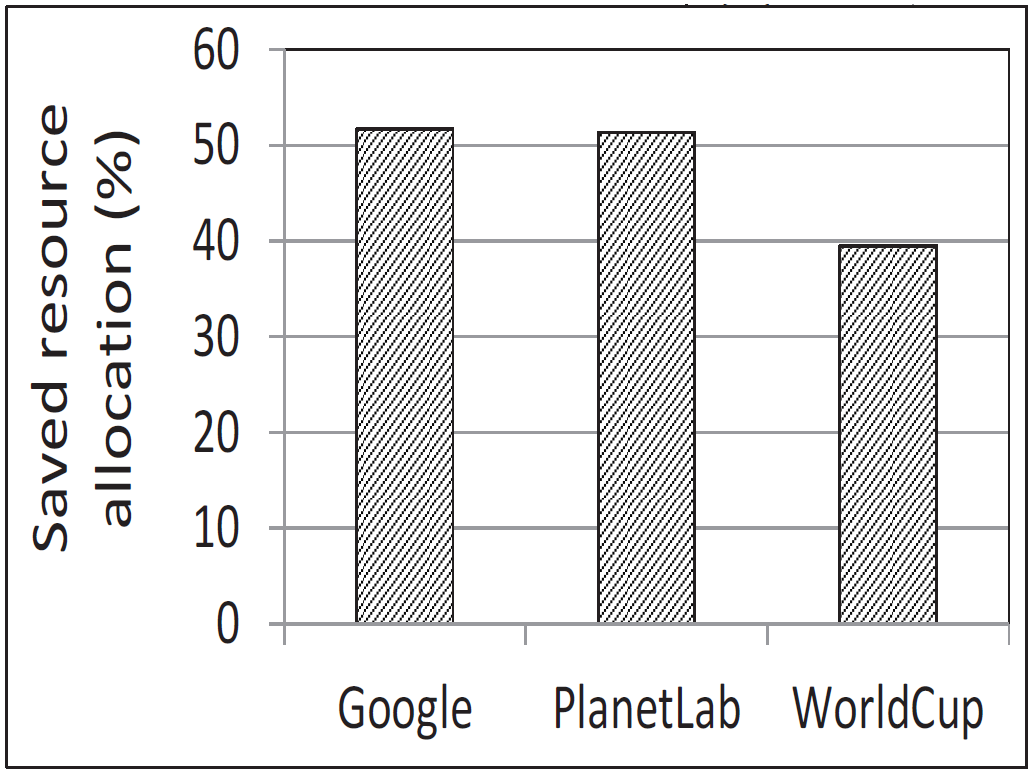
\includegraphics[width=0.7\textwidth]{./figure/eva1_6.PNG}
		\end{figure}
	\end{frame}

% Trace-driven Simulation
\subsection{Trace-driven Simulation}
	\begin{frame}
	\frametitle{Trace-driven Simulation}
		\begin{figure}[h!]
		\centering
		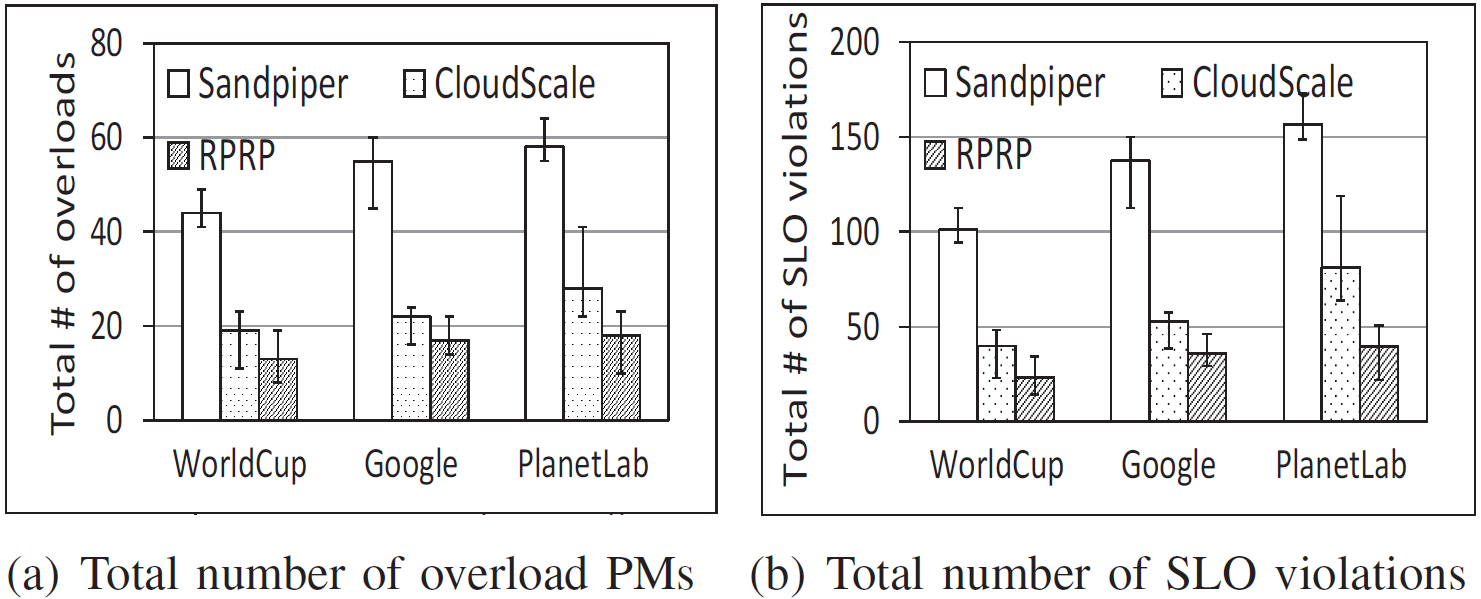
\includegraphics[width=0.7\textwidth]{./figure/eva2_1.PNG}
		\end{figure}
		\begin{figure}[h!]
		\centering
		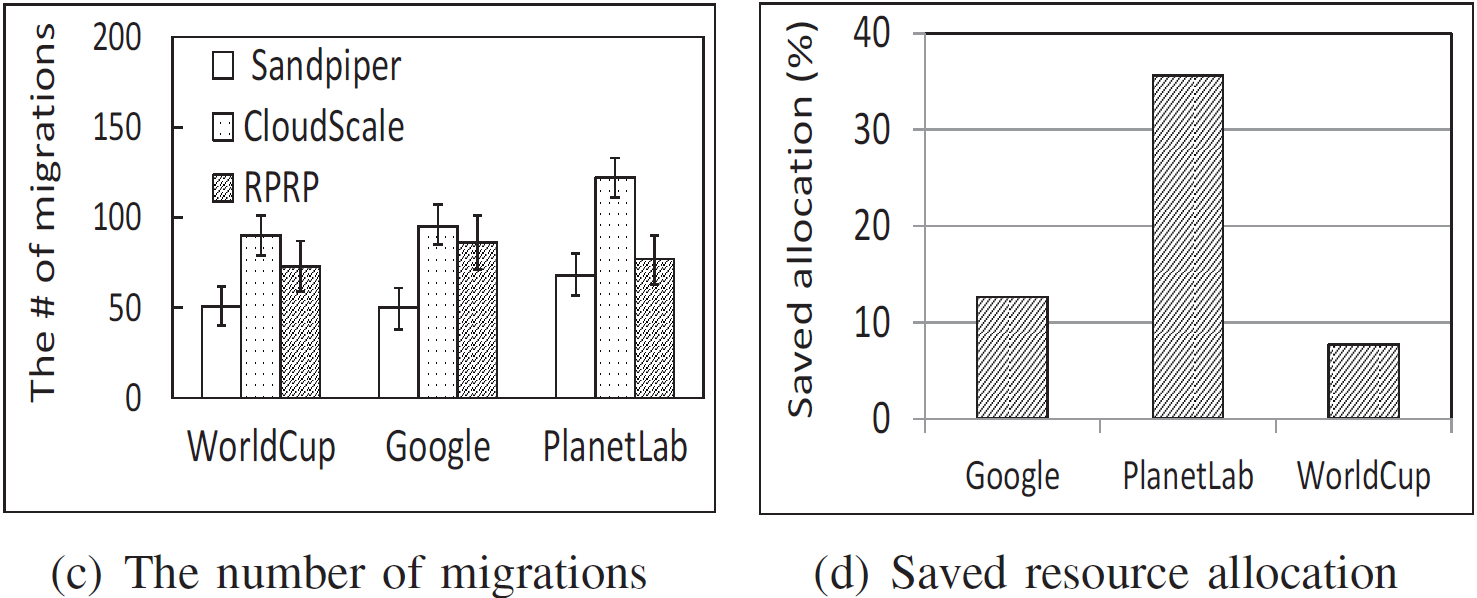
\includegraphics[width=0.7\textwidth]{./figure/eva2_2.PNG}
		\end{figure}
	\end{frame}

% Real-World Testbed Experiments
\subsection{Real-World Testbed Experiments}
	\begin{frame}
	\frametitle{Real-World Testbed Experiments}
		\begin{figure}[h!]
		\centering
		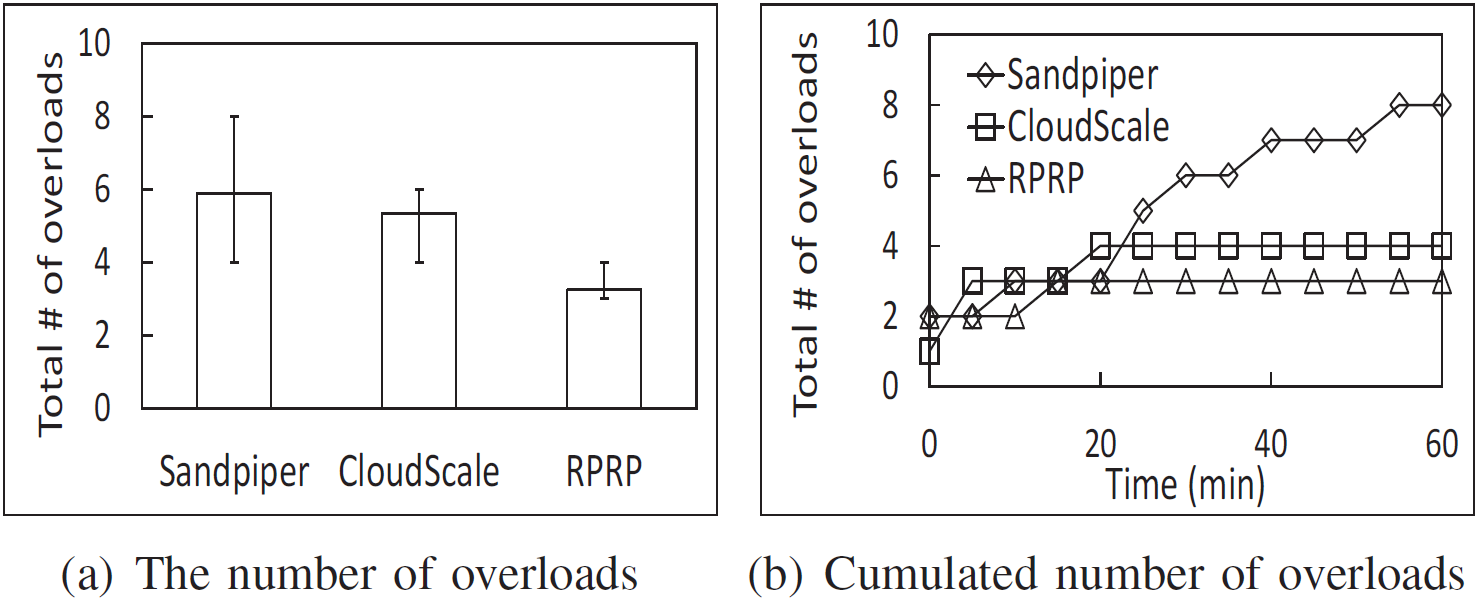
\includegraphics[width=0.7\textwidth]{./figure/eva3_1.PNG}
		\end{figure}
		\begin{figure}[h!]
		\centering
		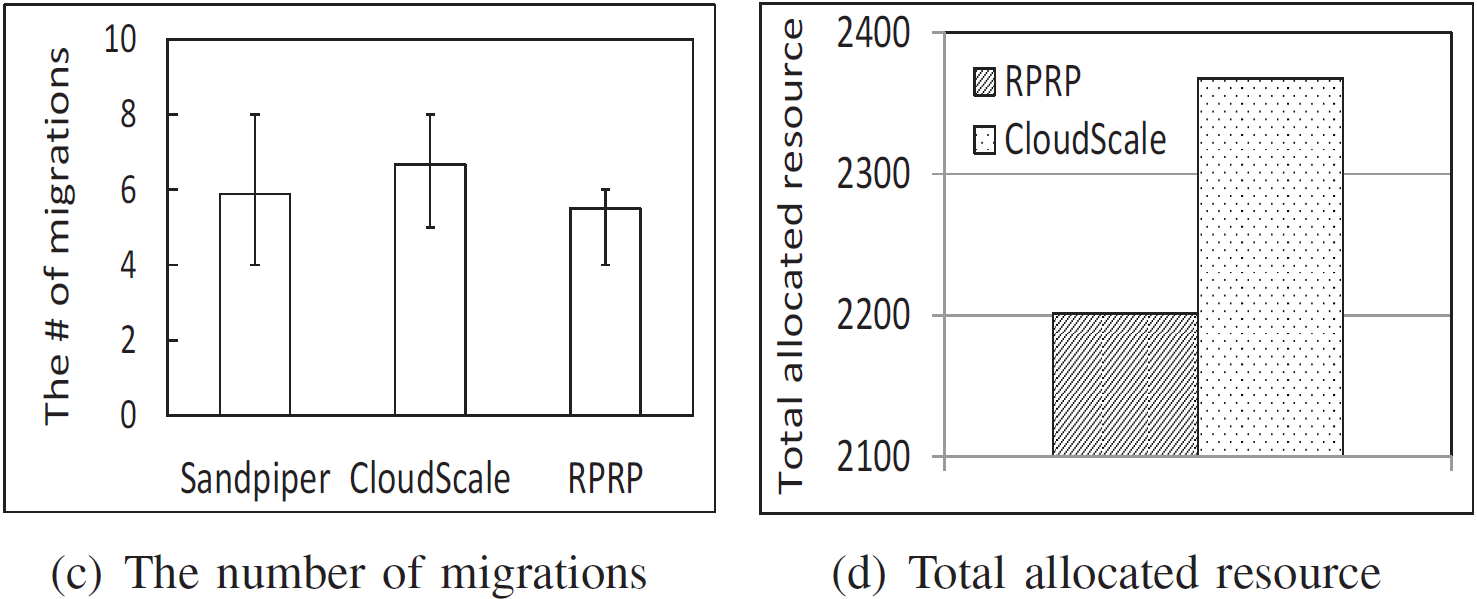
\includegraphics[width=0.7\textwidth]{./figure/eva3_2.PNG}
		\end{figure}
	\end{frame}

%------------------------------------------------
% Conclusion
%------------------------------------------------
\section{Conclusion}

\subsection{Conclusion}
	\begin{frame}
	\frametitle{Conclusion}
		\begin{itemize}
		\item Experimental results show that by using algo. 1 and 2, RPRP reduces 18\% of the allocated resource while reducing 30\% of the total number of SLO violations compared to CloudScale.
		\item These reduced padding values are substantial in improving the resource utilization of a PM that hosts multiple VMs.
		\item RPRP achives higher resource utilization, more accurate demand prediction, and fewer SLO violations than previous schemes.
		\end{itemize}
	\end{frame}

\subsection{Future work}
	\begin{frame}
	\frametitle{Future Work}
		\begin{itemize}
		\item Use the technic mentioned in the paper and the position prediction to make a more accurate prediction in social VR.
		\item Read the referenced paper to research more about the resource scaling method in cloud system.
		\end{itemize}
	\end{frame}

\end{document} 
